%========================%
%        Preamble        %
%========================%
\documentclass[12pt]{amsart}

    %========================%
%        Packages        %
%========================%

\usepackage[utf8]{inputenc}
%\usepackage{amsmath}    % Included in amsart package
%\usepackage{amsthm}     % 
\usepackage{amssymb}      % 
\usepackage{mathtools}      % Paired Limiter Macros
% \usepackage{mdframed}       % boxes for theorem
\usepackage{enumitem}     % Continuous numbering of lists
\usepackage[hidelinks]{hyperref}
\usepackage{tikz}
\usetikzlibrary{positioning}
\usepackage{blindtext}
\usepackage{graphicx}
\usepackage{float}

%========================% 
%          Title         %
%========================% 
\title{Chapters 27 and 28 Notes}
\author{Anish Sundaram}
\date{\today}

%========================% 
%        Theorems        %
%========================% 
\theoremstyle{definition}
\newtheorem{theorem}{Theorem}  % Boxed theorems
\newtheorem{definition}{Definition} % Definitions
\newtheorem{example}{Example}       %
\newtheorem{algorithm}{Algorithm}
\newtheorem*{proof*}{Proof}         % non-numbered
\newtheorem*{remark}{Remark}        %
\numberwithin{equation}{theorem}    % Local equation numbering

\setcounter{tocdepth}{3}      % Show subsubsections in contents

%========================% 
%        Macros          %
%========================% 
\DeclarePairedDelimiter\abs{\lvert}{\rvert}  % Vertical bars
\DeclarePairedDelimiter\norm{\lVert}{\rVert} % Double vertical bars
\newcommand{\drawvec}[1]{                    % matrices on one line
    \begin{bmatrix}
        #1
    \end{bmatrix}
}


% \begin{figure}[H]
%     \centering
%     \includegraphics[width=5in]{global-carbon-cycle.png}
%     \caption{The Global Carbon Cycle}
%     \label{global-carbon-cycle}
% \end{figure}

%========================% 
%         Document       %
%========================% 
\begin{document}

\maketitle

\tableofcontents

\section*{27 Magnetic Field and Magnetic Forces}

But the \textit{fundamental} nature of magnetism is the interaction of moving 
electric charges. Unlike electric forces, which act on electric charges 
whether they are moving or not, magnetic forces act only on \textit{moving charges}.

\subsection*{27.1 Magnetism}

\begin{remark}
    The earth itself is a magnet. Its north geographic pole is close to a magnetic south pole, which is why the north pole of a compass needle points north. The earth’s magnetic axis is not quite parallel to its geographic axis (the axis of ro- tation), so a compass reading deviates somewhat from geographic north. This deviation, which varies with location, is called \textit{magnetic declination or magnetic variation.}
\end{remark}

\begin{remark}
     While isolated positive and negative charges exist, there is no experimental evidence that one isolated magnetic pole exists; poles always appear in pairs. If a bar magnet is broken in two, each broken end becomes a pole 
\end{remark}

\begin{figure}[H]
    \centering
    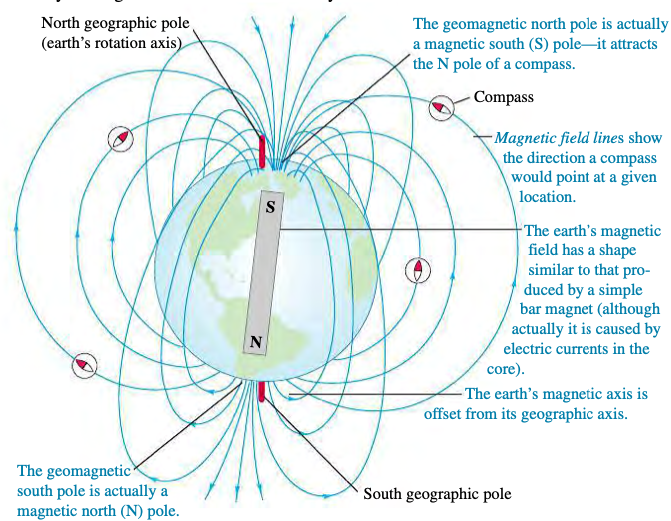
\includegraphics[width=3in]{Media/Magnetism.png}
    \caption{Depiction of Magnetic Field}
    \label{Depiction of Magnetic Field}
\end{figure}

\subsection*{27.2 Magnetic Field}

\begin{definition}
    \textbf{Summary of Electric interactions}:
    \begin{enumerate}
        \item A distribution of electric charge creates an electric field $\vec{E}$ in the surrounding space.
        \item The electric field exerts a force $\vec{F} = q\vec{E}$ on any other charge q that is present in the field.
    \end{enumerate}
\end{definition}

\begin{definition}
    \textbf{Summary of Magnetic interactions}:
    \begin{enumerate}
        \item A moving charge or a current creates a \textbf{magnetic field (B)} in the surrounding
        space (in addition to its \textit{electric} field).
        \item  The magnetic field exerts a force $\vec{F}$ on any other moving charge or current that is present in the field.
    \end{enumerate}

    Magnetic Field strength can be found by the equation 
    $$B = \frac{\mu_0I}{2\pi r}$$ where $\mu_0$ is the permitivity of free space($4\pi \cdot 10^{-7}$ $T\cdot m/A$) and $r$ is the seperation.

    \begin{remark}
        Like electric field, magnetic field is a vector field--that is, a vector quantity associated with each point in space. We will use the symbol $\vec{B}$ for magnetic field.
    \end{remark}
\end{definition}

\begin{figure}[H]
    \centering
    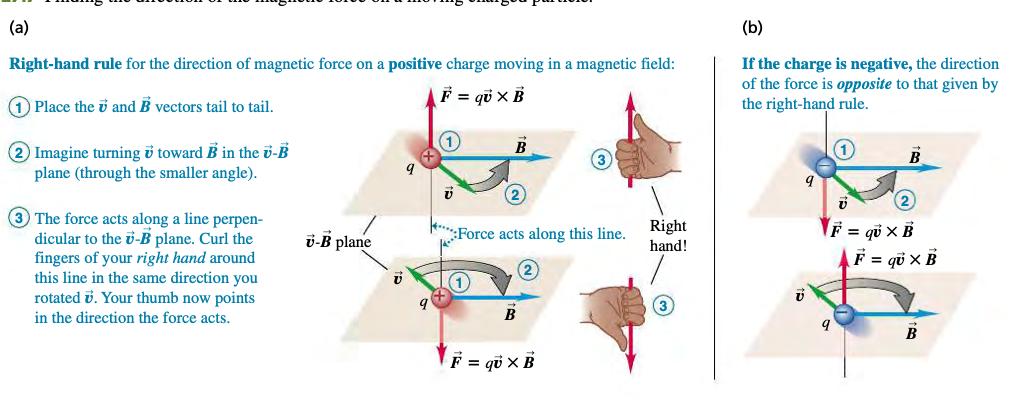
\includegraphics[width=3in]{Media/RHR.png}
    \caption{Right-Hand Rule}
    \label{Right-Hand Rule}
\end{figure}


\subsubsection*{27.2.1 Magnetic Forces on Moving Charges}

\begin{definition}
    \textbf{Key Characteristics of Magnetic Force on Moving Charges}:
    \begin{enumerate}
        \item Force Magnitude is proportional to the magnitude of the charge.
        \item The magnitude of the force is also propor- tional to the magnitude, or “strength,” of the field.
        \item The magnetic force depends on the particle’s
        velocity.
        \item The magnetic force $\vec{F}$ does not have the same direction as the magnetic field $\vec{B}$ but instead is always perpendicular to both $\vec{B}$ and the velocity $\vec{v}$. 
    \end{enumerate}
    The Magnetic force can be found by the equation $$F = |q|v \times B = |q|vBsin\phi$$ where $\phi$ is the angle between the direction of velocity and direction of the magnetic field and the magnitude is measured in teslas ($1T = 1N/A \cdot m$) or in Gauss(1G = $10^{-4}$T)
    \begin{remark}
        The magnetic field of the earth is $10^{-4}$T 1 Gauss.
    \end{remark}
\end{definition}

\begin{remark}
    When a charged particle moves through a region of space where both electric and magnetic fields are present, \textit{both fields exert forces on the particle}. The total force $\vec{F}$ is the vector sum of the electric and magnetic forces: $$\vec{F}=q(\vec{E} + \vec{v}\times \vec{B})$$
\end{remark}

\subsection*{27.3 Magnetic Field Lines and Magnetic Flux}

\begin{definition}
    \textbf{Magnetic Field Lines}:
    Just like an electric field, a magnetic field can be represented through field lines. The more lines there are in a given area the stronger the field , and they never intersect. Magnetic Field Lines are not lines of force, just direction.
\end{definition}

\begin{definition}
    \textbf{Magnetic Flux($\Phi_B$)}:
    A measurement of the total magnetic field which passes through a given area. The total magnetic flux through the surface is the sum of the contributions from the individual area elements. Can be found using the following equation:
    $$\Phi_B = \int B cos\phi dA = \int\vec{B}\cdot d \vec{A}$$
    Magnetic Flux is scalar and its units are Weber(1 Wb = 1 $T\cdot m^2$ = 1 $N\cdot m/A$)

\end{definition}

\subsection*{27.4 Motion of Charged Particles in a Magnetic Field}

\begin{remark}
    Motion of a charged particle under the action of a magnetic field alone is always motion with constant speed.
\end{remark}

\begin{remark}
    When velocity and magnetic field are perpendicular, the particle exhibits circular motion. This relation is shown by $$F = |q|vb = m\frac{v^2}{R}$$ whose radius can be found by $$R = \frac{mv}{|q|B}$$ and whose angular speed can be found by $$\omega = \frac{v}{r} = \frac{|q|B}{m}$$
\end{remark}

\subsection*{27.5 Applications of Motion of Charged Particles}

\subsubsection*{27.5.1 Velocity Selector}

\begin{definition}
    \textbf{Velocity Selector}:
    An arrangement of electric and magnetic fields that can be used to select 
    only particles of a specific speed. Only particles with speed equal to 
    E/B can pass through without being deflected, and this process works for 
    electrons and protons.
\end{definition}

\begin{figure}[H]
    \centering
    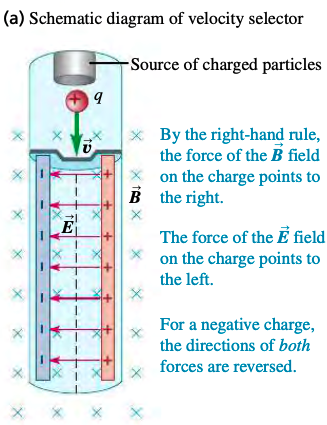
\includegraphics[width=3in]{Media/Velsec.png}
    \caption{Model of Velocity Selector}
    \label{Model of Velocity Selector}
\end{figure}

\subsection*{27.6 Magnetic Force on a current-carrying Conductor}

\begin{remark}
    Magnetic fields are caused by moving charges, and thus exist around a current
    carrying wire. We can manipulate the equation for single charges for currents,$\vec{F}=|q|vBsin\phi$, by factoring that the total force would be the force per charge multiplied by the amount of charges in the wire:
    $$\vec{F}=|q|vBsin\phi = (nAl)(qvBsin\phi) = IlBsin\phi$$ 
    and for infinitesmal wire segments: 
    $$d\vec{F} = Id\vec{l} \times \vec{B}$$
\end{remark}

\begin{figure}[H]
    \centering
    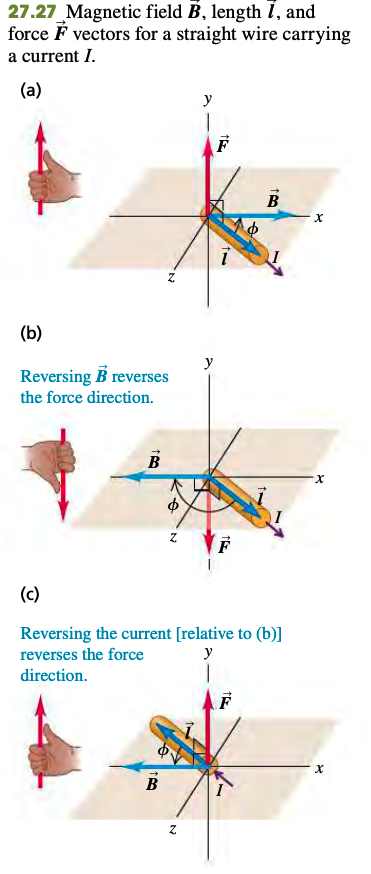
\includegraphics[width=3in]{Media/wirerhr.png}
    \caption{Right-Hand Rule for a Current-Carrying Wire}
    \label{Right-Hand Rule for a Current-Carrying Wire}
\end{figure}

\subsection*{27.7 Force and Torque on a Current Loop}
\begin{remark}
    The net force on a current loop in a uniform magnetic field is zero. However, the net torque is not in general equal to zero.
\end{remark}

\begin{definition}
    \textbf{Torque on a Current Loop ($\tau$)}:
    In a uniform field the total force is zero but torque is not necessary, as in a dipole. The magnitude of the magnetic torque can be found using the equation $$\tau = IBAsin\phi$$ where A is the area of the loop within the field and $\phi$ is the area normal to loop plane and field direction.
\end{definition}

\begin{definition}
    \textbf{Magnetic Dipole Moment($\mu$)}:
    Also called the \textbf{Magnetic Moment}, this is the product $IA$ and is analogous to the electric dipole moment by having a north and south poles. A current loop or any body that experiences a magnetic torque is called a \textbf{Magnetic Dipole}.
\end{definition}

\subsubsection*{27.7.1 Potential Energy for a Magnetic Dipole}

\begin{definition}
    \textbf{Potential Energy for a Magnetic Dipole(U)}:
    When a dipole changes orientation the field does work on it. Because potential energy is the negative of total work, the equation for finding U is the parallel of the potential energy in an electric field: 
    $$U = -\vec{\mu}\cdot \vec{B} = -\mu Bcos\phi$$
    where $\phi$ is the angle between $\mu$ and B.
\end{definition}

\subsubsection*{27.7.2 Magnetic torque: Loops and Coils}

\begin{definition}
    \textbf{Solenoid}:
    A helical winding of wire, such as a coil wound on a circular cylinder. The total torque on a solenoid in a megnetic field is the sum of the torques of the individual turns, or $$\tau = NIABsin\phi$$ where $\phi$ is the angle between the axis of the solenoid and the direction of the field.
\end{definition}

\subsection*{27.8 Direct-Current Motor}

\begin{definition}
    \textbf{Parts of Motor}:
    The moving part of the motor is the \textit{rotor}, a length of wire formed into an open-ended loop and free to rotate about an axis. The ends of the rotor wires are attached to circular conducting segments that form a \textit{commutator}.
\end{definition}
\begin{figure}[H]
    \centering
    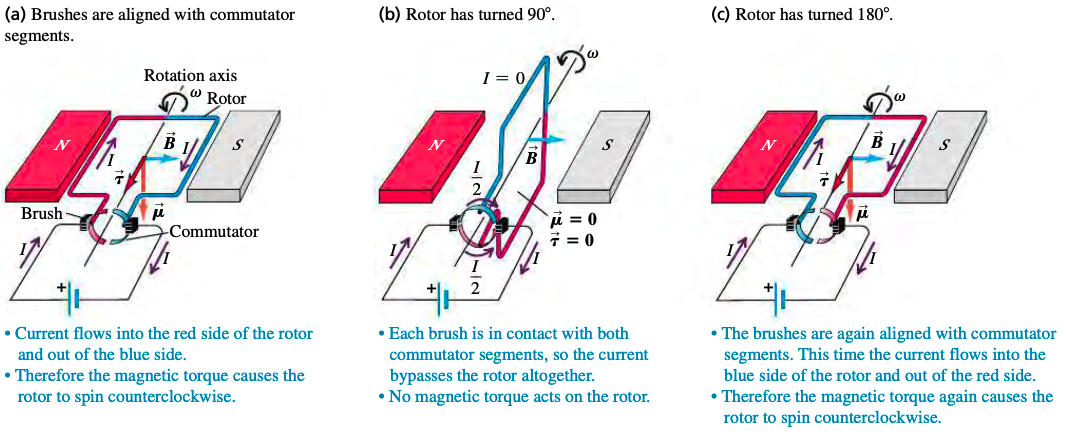
\includegraphics[width=3in]{Media/motor.png}
    \caption{Model of a Motor}
    \label{Model of a Motor}
\end{figure}
\begin{remark}
    In a dc motor a magnetic field exerts a torque on a current in the rotor. Motion of the rotor through the magnetic field causes an induced emf called a back emf. For a series motor, in which the rotor coil is in series with coils that produce the magnetic field, the terminal voltage is the sum of the back emf and the drop $Ir$ across the internal resistance.
\end{remark}

\subsection*{27.9 The Hall Effect}

\begin{definition}
    \textbf{The Hall Effect}:
    A potential difference perpendicular to the direction of current in a conductor, when the conductor is placed in a magnetic field. The Hall potential is determined by the requirement that the associated electric field must just balance the magnetic force on a moving charge. Hall-effect measurements can be used to determine the sign of charge carriers and their concentration n. 
    $$nq=\frac{-J_xB_y}{E_z}$$


\end{definition}


\section*{28 Sources of Magnetic Field}

\end{document}